\newpage
\changeindent{0cm}
\section{要素技術}
\changeindent{2cm}

本章では,実験に関連する要素技術について説明する.

\changeindent{0cm}
\subsection{半教師あり学習}
\changeindent{2cm}
半教師あり学習 (Semi Supervised Learning: SSL)\cite{zhu2005semi} は
大量のラベルなしデータと少量のラベル付きデータを用いて学習を行う手法である.

\changeindent{0cm}
\subsection{疑似ラベル}
\changeindent{2cm}
疑似ラベル (Pseudo Label)\cite{lee2013pseudo} はあるモデルによって予測されるラベルなしデータに対する暫定的なラベルである.
 SSL では疑似ラベルを付与したデータをラベル付きデータに混ぜて学習することで各ラベル同士に対する確率分布を粗密なものとして作用することで正則化の役割をする.
 

\changeindent{0cm}
\subsection{SimCLR}
\changeindent{2cm}
Simple framework for Contrastive Learning of visual Representation(SimCLR)\cite{chen2020simple} は SSL の一つである.
図\ref{fig:SimCLR}に概略図を示す.モデルの構造は Encoder,Projection Head,Classsifer
から構成されており, Encoder と Projection Head に対して,全データを用いて Contrastive Learning によって学習する.次に学習済みの Encoder と Classifer に対して,ラベル付きデータを用いて Classfier の学習を行う.最後にモデルの蒸留を行うことで最終的なモデルを得る.
\begin{figure}[h]
	\begin{center}
		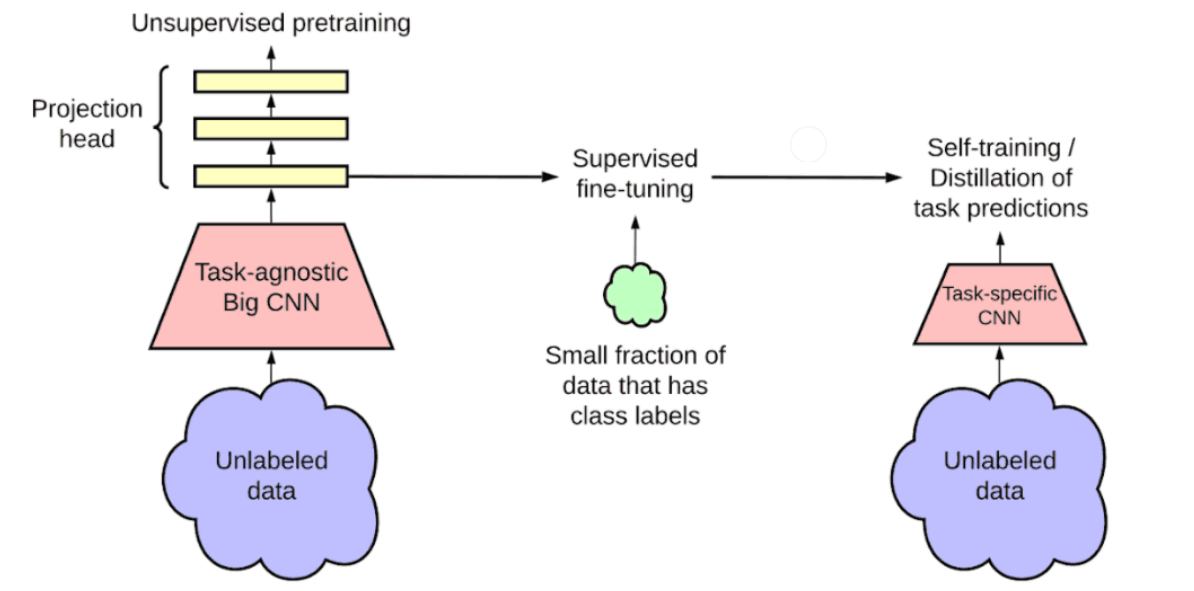
\includegraphics[scale=1.0]{./images/SimCLR.png}
		\caption{SimCLR の概略: 文献\cite{chen2020big}の Figure 3 を参照\label{fig:SimCLR}}
	\end{center}
\end{figure}

\changeindent{0cm}
\subsubsection{Cotrastive Learning}
\changeindent{2cm}
Contrastive Learning (CL)\cite{tian2020makes} とは特徴表現を獲得するための
自己教師あり学習のひとつである.
ある画像変換をした画像のペアについて元画像が一致するか否かを識別するタスクであり,
一つの画像から得られる特徴表現が画像変換によって
画像の持つ意味が大きく変化させない変形を獲得することができる.
具体的な方法について,バッチ内の画像枚数を $N$ 枚とすると, Data Augmentation によって2倍に増やしたとき,
各画像に対して正例は1枚,負例は $2(N-1)$ 枚となる.このとき特徴ベクトル間の距離として cos 類似度を用いて
式となる.また,正例との距離を小さくかつ,負例との距離を大きくするために正例のペア $(z_i,z_j)$ に対するロス $l_{i,j}$ は式で表され,
バッチ全体のロス $L$ 


\changeindent{0cm}
\subsection{ResNet}
\changeindent{2cm}
Residual Network (: ResNet)\cite{he2016deep} は Deep Neural Network (: DNN) のモデルの一つであり,
 DNNにおいて層を深くすることで発生する劣化問題及び勾配消失問題を解消するために残差についての学習を行うことを目的としている.図\ref{fig:ResBlock}に ResNet の構成要素である Residual Block の構造を示す.
2層の畳み込み層とショートカットの足し合わせた構造となっている.

\begin{figure}[h]
	\begin{center}
		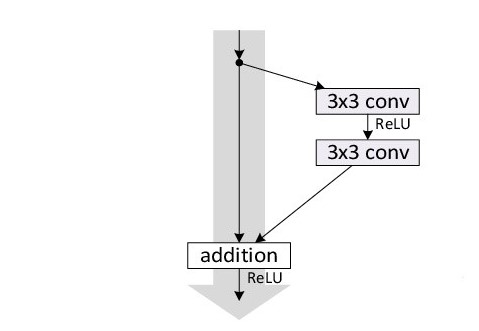
\includegraphics[scale=0.5]{./images/ResBlock.jpg}
		\caption{Residual Block の構造: 文献\cite{he2016identity}の Figure 2.(a) を参照\label{fig:ResBlock}}
	\end{center}
\end{figure}

\changeindent{0cm}
\subsection{Genetic Algorithm}
\changeindent{2cm}
\cite{whitley1994genetic}


\cite{murata1996multi}



CIFAR10\cite{krizhevsky2009learning}